%\documentclass[12pt]{beamer}
%\usetheme{Boadilla}
\documentclass[aspectratio=169, compress, xcolor=table,xcolor=dvipsnames]{beamer}

%\usepackage{graphicx,hyperref,url}
%\usepackage{color}

\setbeamercolor{structure}{fg=Brown} %, bg=YellowOrange}
\usetheme{Goettingen}

\setbeamercolor{palette sidebar secondary}{fg=Blue} %yellow,bg=blue}
\setbeamercolor{section in sidebar shaded}{fg=Black} %,bg=Brown}

%\usetheme{Goettingen}
%\usetheme{Madrid}
%\usecolortheme{crane}
\usecolortheme{orchid}


%\useoutertheme{infolines} % Alternatively: miniframes, infolines, split
\useinnertheme{circles}

\setbeamertemplate{footline}[frame number]
\setbeamerfont{page number in head/foot}{size=\large}

\usepackage[utf8]{inputenc}
\usepackage[british]{babel}
\usepackage{amsmath}
\usepackage{amsfonts}
\usepackage{amssymb}
\usepackage{graphicx}
\usepackage[noend]{algpseudocode}

%\usepackage{natbib} % Harvard style referencing
%\bibliographystyle{agsm}

\author{Kamal Bentahar}
\title{Investigating 3SAT}
\subtitle{(Guide presentation for 380CT Coursework 2)}
\date{\today}

\setbeamercolor{math text}{fg=blue}
\setbeamercovered{transparent}
\setbeamertemplate{navigation symbols}{}

%%%%

\newcommand{\cp}{\textbf{P}}
\newcommand{\cnp}{\textbf{NP}}
\newcommand{\cnpc}{\textbf{NP-complete}}
\newcommand{\cnph}{\textbf{NP-hard}}

%%%%

\begin{document}

\begin{frame}[noframenumbering]
	\titlepage
\end{frame}
	
\begin{frame}{Notation}
	Let $x_1,x_2,\ldots,x_n$ be Boolean \textbf{variables}, and let $\phi$ be a Boolean formula written in 3-cnf (Conjunctive Normal Form)
	\[
	\phi = c_1\land c_2\land \cdots \land c_\ell,
	\]
where each \textbf{clause} $c_m=x_i\lor x_j\lor x_k$, for some $i,j,k=1,2,\ldots,n$ and $m=1,\ldots,\ell$.

\vfill
A \textbf{literal} can be $x_i$ or $\lnot x_i$ for some $i=1,2,\ldots,n$.

\vfill
The ratio $\ell/n$ is important for experiments, and will be denoted by $\rho$.
\end{frame}

\begin{frame}{Definition of the problem}

%Let $\phi$ be a Boolean expression given in 3-cnf form.

	\begin{block}{Decisional 3SAT}
		Decide if $\phi$ is satisfiable.
	\end{block}
	\cnpc.

	\begin{block}{Computational/Search 3SAT}
		If $\phi$ is satisfiable then find a satisfying assignment.
	\end{block}

	\begin{block}{Optimization 3SAT (Max 3SAT)}
		Find an assignment that minimizes the number of non-satisfying clauses.
	\end{block}
	\cnph.
\end{frame}

\begin{frame}
{Testing methodology}

\begin{enumerate}
	\item \textbf{Exhaustive search:} average time for instances with increasing $n$.
	\item \textbf{Dynamic programming:} average time for instances with increasing $\ell$.
	\item \textbf{Greedy and meta-heuristics:} quality of approximation with increasing $\rho$ . Quality of approximation is calculated as the ratio of satisfied clauses to $\ell$.
\end{enumerate}
\end{frame}

\begin{frame}
{Random instances sampling strategy}
%{Sampling strategy}

General 3SAT instances will be generated by selecting exactly 3 different literals from
\[\{x_1, \lnot x_1, x_2, \lnot x_2, \ldots, x_n\, \lnot x_n\}\]
uniformly at random.
Do not allow clauses including both $x_i$ and $\lnot x_i$ (tautological clauses).
\cite{sls book}.

\vfill

For `yes' instances, a random variable assignment is fixed first, then clauses are randomly constructed making sure each is satisfiable.

\end{frame}

%
%
% -------------------------------------------------------------------------------------------------------------------
%
%

\section{Exact methods}
\subsection{Exhaustive}

\begin{frame}
{Exhaustive search -- theory}

\begin{algorithmic}[1]\sffamily
\For{all possible variable assignments of $x_1,x_2,\ldots,x_n$}
	\If {$\phi(x_1,x_2,\ldots,x_n)$ evaluates to True}
	\State {\Return True}
	\EndIf
\EndFor
\State \Return False
\end{algorithmic}

\vfill

There are $2^n$ possible assignments, and each  evaluation of $\phi$ costs $O(\ell)$. So this algorithm costs \[O(\ell\, 2^n).\]
\end{frame}

\begin{frame}
{Exhaustive search -- empirical results}

\begin{center}
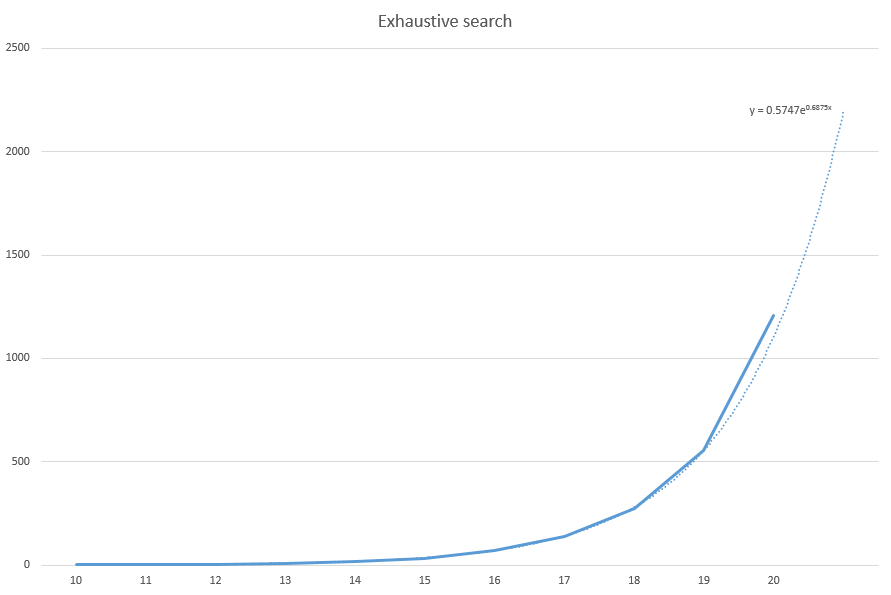
\includegraphics[width=0.7\textwidth]{img/exh2}
\end{center}

Average time in $100\times$ seconds [TODO: REDO EXPERIMENT] for randomly generated instances with $n=\ell$ for $n=10,\ldots$.

Dotted line: fitted exponential curve.

\end{frame}

%
%
% -------------------------------------------------------------------------------------------------------------------
%
%

\subsection{Dynamic}

\begin{frame}
{Dynamic Programming}

\begin{algorithmic}[1]\sffamily
	\State $\cal A\gets\emptyset$
		\Comment Set of possible assignments
	\For{$k=1,2,\ldots,\ell$}
		\State $S\gets$ all the satisfying assignments of $c_k$
			\Comment 7 at most
		\State $update \gets \emptyset$
		\For{$p\in \cal A$}
			\For{$\sigma\in S$}
				\If {$\sigma$ and $p$ do not clash}
					\State join $p$ and $\sigma$ and append to $update$
				\EndIf
			\EndFor
		\EndFor
		\State ${\cal A}\gets update$
	\EndFor
	\State \Return best candidate in $\cal A$
\end{algorithmic}

\bigskip
\vfill

Cost: $O(\ell\times \max |\cal A|)$ time and $O(\max |\cal A|)$ space, but $|\cal A|$ can grow like $7^k$ in the worst case, we deduce that this algorithm can cost
\[O(\ell 7^\ell) \text{ time, and } O(7^\ell)\text{ space}\]

Only useful if $\ell$ is small.
[TODO: VERIFY. CAN COST BE REDUCED?]
\end{frame}

\begin{frame}
	{Dynamic Programming -- empirical results}

[TODO]

\end{frame}

\subsection{Discussion}

\begin{frame}
{Exact methods -- discussion of results}

[TODO]
\end{frame}

%
%
% -------------------------------------------------------------------------------------------------------------------
%
%

\section{Approximation}

\subsection{Greedy}

\begin{frame}
{Greedy -- theory}

Find the variable that appears most often and assign it accordingly to maximize ...

%        variables_occurance = [[i,0] for i in range(-self.nv,self.nv+1)] # if i != 0]
%        for c in self.clauses:
%	        for v in c:
%		        variables_occurance[ v+self.nv ][1] += 1
%        variables_occurance.sort( key=lambda a:a[1] ) #, reverse=True )
%        for v in variables_occurance:
%	        self.variable_assignment[ abs(v[0])-1 ] = (v[0]>0)
%        return self.ratio_satisfied()

\begin{algorithmic}[1]\sffamily
	\State $L \gets \emptyset$
	\For{$w\in\{x_1,\lnot x_1,\ldots,x_n,\lnot x_n\}$}
		\State Count occurrences of $w$ in $\phi$
		\State Append pair $(w, \text{count of occurrences of $w$ in $\phi$})$ to $L$
	\EndFor
	\State Sort $L$ with respect to the second component
%	\State\Comment{We now have the literals in decreasing order of total occurrence}
	\For{$(w,c)\in L$}
		\State Set $w$ to True \Comment{If $w=\lnot x_i$ then set $x_i$ to False}
	\EndFor
	\State \Return count of satisfied clauses
\end{algorithmic}

\vfill

Cost: $O(n\log n)$ assuming the use of an $O(n\log n)$ sorting algorithm.
\end{frame}

\begin{frame}
{Greedy method -- empirical results}
\begin{center}
	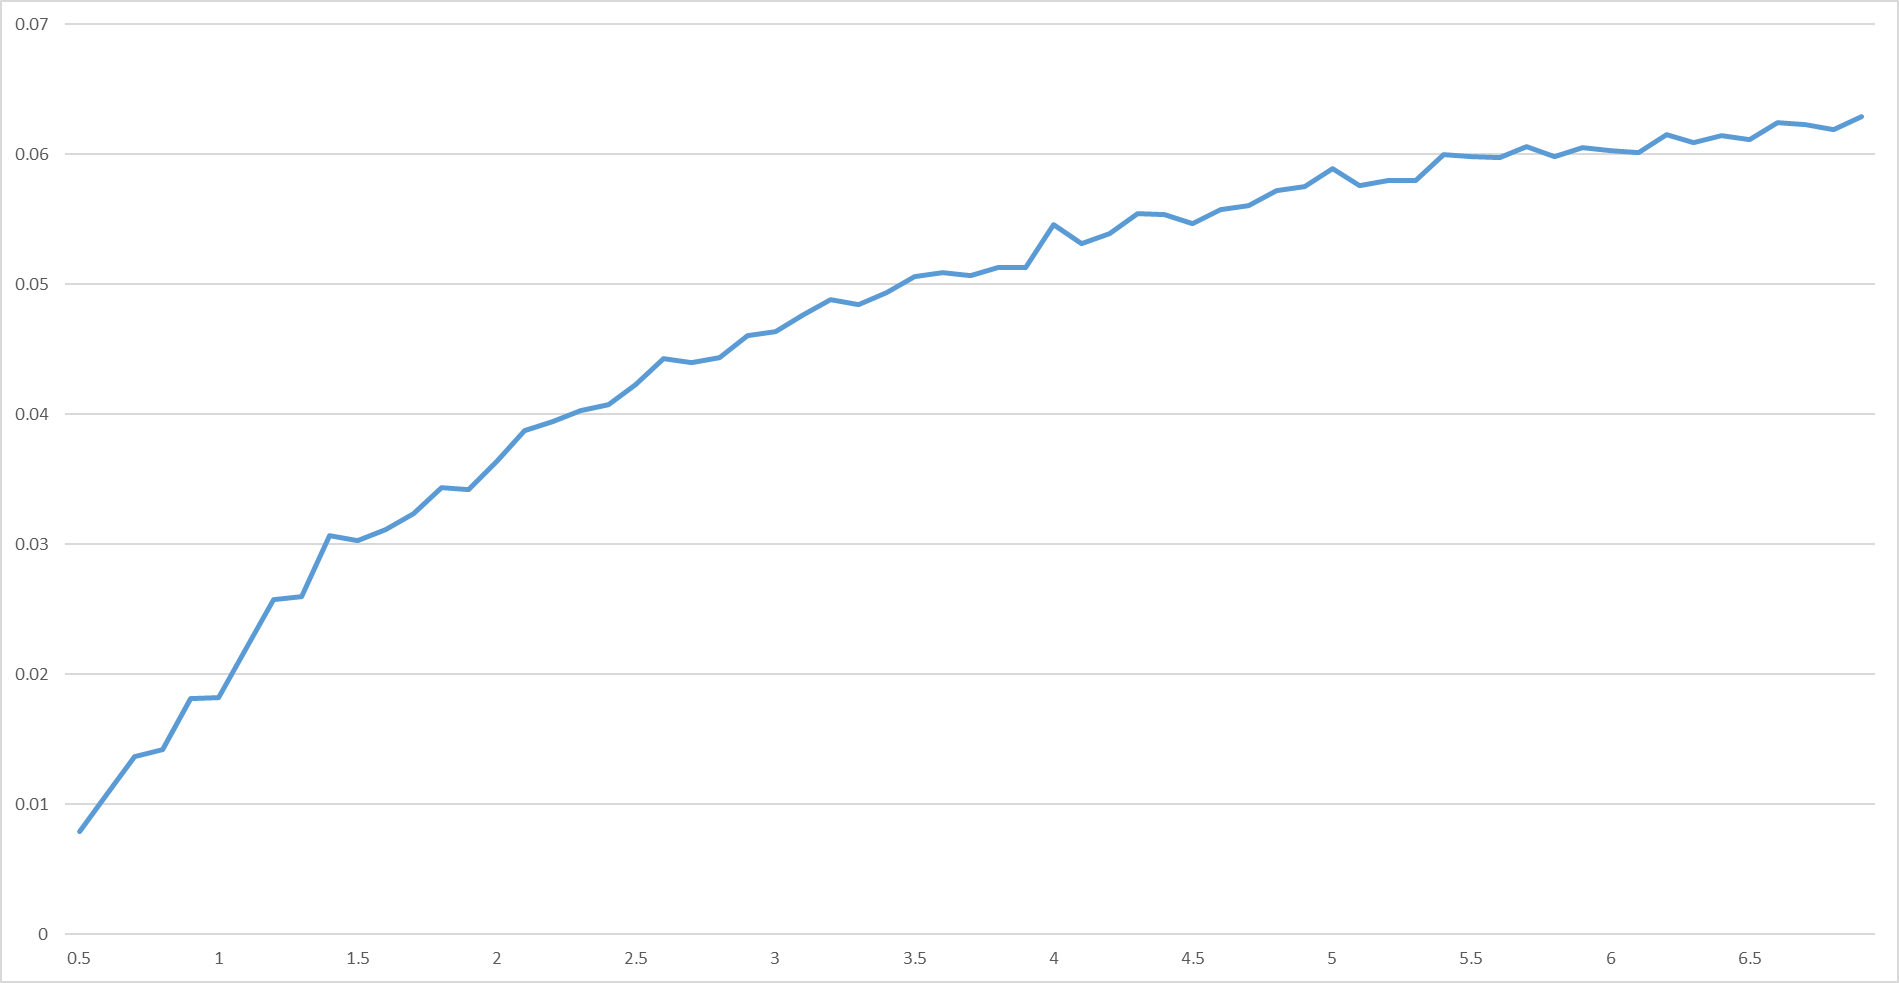
\includegraphics[width=\textwidth]{img/greedy}
\end{center}

Average ratio of clauses unsatisfied by Greedy for $\rho=0.5,\ldots,7$.
\end{frame}

%
%
% -------------------------------------------------------------------------------------------------------------------
%
%

\subsection{GRASP}

\begin{frame}
{GRASP -- theory}

\begin{algorithmic}[1]\sffamily
	\State $best\_candidate\gets \emptyset$
	\While{(termination condition is not met)}
	\State{$greedy\_candidate\gets \text{ConstructGreedyRandomizedSolution}()$}
	\State{$grasp\_candidate\gets \text{LocalSearch}(greedy\_candidate)$}
	\If{$f(grasp\_candidate)<f(best\_candidate)$}
	\State{$best\_candidate\gets grasp\_candidate$}
	\EndIf
	\EndWhile
	\State\Return{$best\_candidate$}
\end{algorithmic}

\vfill

\begin{itemize}
	\item ``termination condition'' is simply to repeat a fixed number of times, e.g. 100 times.
	\item $f$ gives the ratio of unsatisfied clauses to $\ell$. Objective is to minimize it.
	\item $ConstructGreedyRandomizedSolution()$ works like Greedy but shuffles $L$ in blocks of a given size. [TODO: EXPLAIN MORE]
	\item $LocalSearch()$ works by flipping the variables' assignment.
\end{itemize}
\end{frame}%

\begin{frame}
	{GRASP -- empirical results}

\begin{center}
	\includegraphics[width=0.9\textwidth]{img/grASP}
\end{center}

Results for $\rho=0.5,\ldots,7$ and $n=20$.
\end{frame}

%
%
% -------------------------------------------------------------------------------------------------------------------
%
%

\subsection{ACO}

\begin{frame}
{Ant Colony Optimization -- theory}

	\begin{algorithmic}[1]\sffamily
		\State initialize weights
		\While{termination criterion is not satisfied}
		\State generate population $sp$ of candidate solutions using subsidiary randomized constructive search
		\State perform subsidiary local search on $sp$
		\State adapt weights based on $sp$
		\EndWhile
		\State\Return{$s$}
	\end{algorithmic}
	The subsidiary constructive search uses weights (pheromone trails) and heuristic information.


\end{frame}

\begin{frame}
	{Ant Colony Optimization -- empirical results}
\end{frame}

\subsection{Discussion}

\begin{frame}
	{Approximation methods -- discussion of results}
	
	[TODO]
\end{frame}

%
%
% =======================================================================
%
%

\section{Special cases}

\begin{frame}
{Special cases}

\begin{enumerate}
	\item $n=1$. If $x$ and $\lnot x$ appear in the same clause then it becomes a tautology, and the clause can be ignored. Otherwise $x\lor x\lor x = x$ and $\lnot x\lor \lnot x\lor \lnot x = \lnot x$. So $\phi$ simplifies to a conjunction of terminals, whose satisfiability is easy to establish. [TODO: details?]
	\item $n=2$. We get 2-SAT which is in \cp. [TODO: details?]
	\item $\ell=1$. Always satisfiable. [TODO: true for $\ell\leq n$?]
\end{enumerate}

\end{frame}
%
%
% =======================================================================
%
%

\section{Conclusion}

\begin{frame}
{Conclusion}

\begin{itemize}
	\item If instance is a special case then can be solved in polynomial time.
	\item Exhaustive search useful when $n$ is small.
	\item Dynamic programming useful when $\ell$ is small.
	\item Otherwise, use GRASP, ACO, or other metaheuristics for approximate solutions.
\end{itemize}
\end{frame}
%
% ------------
%

\section{Reflection}

\begin{frame}
	{Reflection}

\end{frame}

\begin{frame}
{References}
	
	\begin{thebibliography}{References}
		\beamertemplatebookbibitems
		\bibitem{sls book}
		Hoos, H. and Stutzler, T. (2005)
		\textbf{Stochastic Local Search: Foundations and Applications.}
		Morgan Kaufmann

		\bibitem{guide}
		Garey, S. and Johnson, D. (1979)
		\textbf{Computers and Intractability: A Guide to the Theory of NP-Completeness.}
		Freeman
				
	\end{thebibliography}
	
\end{frame}

\end{document}